%%%%%%%%%%%%%%%%%%%%%%%%%%%%%%%%%%%%%%%%%%%
%%%%%

%% Preamble

\documentclass[12pt]{article}
\usepackage{geometry}
\geometry{a4paper}
\usepackage[]{listings}
\usepackage[]{color}
\usepackage[]{enumerate}

% Solarized palette
\definecolor{solarizedBase03}{RGB}{0,43,54}
\definecolor{solarizedBase02}{RGB}{7,54,66}
\definecolor{solarizedBase01}{RGB}{88,110,117}
\definecolor{solarizedBase00}{RGB}{101,123,131}
\definecolor{solarizedBase0}{RGB}{131,148,150}
\definecolor{solarizedBase1}{RGB}{147,161,161}
\definecolor{solarizedBase2}{RGB}{238,232,213}
\definecolor{solarizedBase3}{RGB}{253,246,227}
\definecolor{solarizedYellow}{RGB}{181,137,0}
\definecolor{solarizedOrange}{RGB}{203,75,22}
\definecolor{solarizedRed}{RGB}{220,50,47}
\definecolor{solarizedMagenta}{RGB}{211,54,130}
\definecolor{solarizedViolet}{RGB}{108,113,196}
\definecolor{solarizedBlue}{RGB}{38,139,210}
\definecolor{solarizedCyan}{RGB}{42,161,152}
\definecolor{solarizedGreen}{RGB}{133,153,0}

%% Style definition for code highlighting
\lstdefinestyle{highlight}{
    %%backgroundcolor=\color{solarizedBase3},   
    commentstyle=\color{solarizedBase1},
    keywordstyle=\color{solarizedBlue},
    numberstyle=\tiny\color{codegray},
    stringstyle=\color{solarizedGreen},
    basicstyle=\ttfamily\color{solarizedBase01},
    breakatwhitespace=false,         
    breaklines=true,                 
    captionpos=t,                    
    keepspaces=true,                 
    numbers=left,                    
    numbersep=5pt,                  
    showspaces=false,                
    showstringspaces=false,
    showtabs=false,                  
    tabsize=2,
    xleftmargin=.05\textwidth
}

%% Define the line number styles. 
 \definecolor{codegray}{rgb}{0.5,0.5,0.5}

%% Set default style for lstdefine
\lstset{style=highlight}

%% Settings for Fonts, comment out so that Apple only fonts don't break Linux build.
\usepackage{fontspec,xltxtra,xunicode}
\defaultfontfeatures{Mapping=tex-text}



%% Start Article
\title{Computational Lab Group Project\\Journal}
\author{Laurynas Mince}

\begin{document}
\maketitle

\section*{Friday, 30 January 2015}

Today I have done the following:
\begin{enumerate}
	\item Improved the \textsc{Gnuplot} script to plot the equipotential lines. The script and its output can be found at the end of this entry.
	\item Fixed some problems in Martynas' code to generate a data to plot an electric field. 
\end{enumerate}

\subsection*{Appendix}
%%%%%%%%%%%%%%%%%%
%%% Gnuplot script to plot equipotential lines
\lstinputlisting[language=Gnuplot, caption=Gnuplot script to plot the equipotential lines of the numerical solution to the problem A, label=lst:jan301]{./Jan30/equipotential.plot}
%%%%% Output of the above script
\begin{figure}
	\centering
	\caption{Plot of the equipotential lines. Solution of the problem A using numerical techniques.}
	\label{fig:jan301}
	\includegraphics[scale=0.7, angle=-90]{./Jan30/equipotential.eps}
\end{figure}

\end{document}